\documentclass{beamer}

\usepackage{amssymb,amsmath}
\usepackage{graphicx}
\usepackage{url}
\usepackage{color}
\usepackage{relsize}		% For \smaller
\usepackage{url}			% For \url
\usepackage{epstopdf}	% Included EPS files automatically converted to PDF to include with pdflatex
\usepackage{pagenote}[continuous,page]

%For MindMaps
% \usepackage{tikz}%
% \usetikzlibrary{mindmap,trees,arrows}%

%%% Color Definitions %%%%%%%%%%%%%%%%%%%%%%%%%%%%%%%%%%%%%%%%%%%%%%%%%%%%%%%%%
%\definecolor{bordercol}{RGB}{40,40,40}
%\definecolor{headercol1}{RGB}{186,215,230}
%\definecolor{headercol2}{RGB}{80,80,80}
%\definecolor{headerfontcol}{RGB}{0,0,0}
%\definecolor{boxcolor}{RGB}{186,215,230}

%%% Save space in lists. Use this after the opening of the list %%%%%%%%%%%%%%%%
%\newcommand{\compresslist}{
%	\setlength{\itemsep}{1pt}
%	\setlength{\parskip}{0pt}
%	\setlength{\parsep}{0pt}
%}

%\setbeameroption{show notes on top}

% You should run 'pdflatex' TWICE, because of TOC issues.

% Rename this file.  A common temptation for first-time slide makers
% is to name it something like ``my_talk.tex'' or
% ``john_doe_talk.tex'' or even ``discrete_math_seminar_talk.tex''.
% You really won't like any of these titles the second time you give a
% talk.  Try naming your tex file something more descriptive, like
% ``riemann_hypothesis_short_proof_talk.tex''.  Even better (in case
% you recycle 99% of a talk, but still want to change a little, and
% retain copies of each), how about
% ``riemann_hypothesis_short_proof_MIT-Colloquium.2000-01-01.tex''?

\mode<presentation>
{
  % A tip: pick a theme you like first, and THEN modify the color theme, and then add math content.
  % Warsaw is the theme selected by default in Beamer's installation sample files.

  %%%%%%%%%%%%%%%%%%%%%%%%%%%% THEME
  %\usetheme{Madrid}		% No subsection
  \usetheme{AnnArbor}  % Subsection on top, no color


  %\usetheme{Antibes}
  %\usetheme{Bergen}
  %\usetheme{Berkeley}		% bem bacana - menu esquerdo
  %\usetheme{Berlin}
  %\usetheme{Boadilla}
  %\usetheme{boxes}
  %\usetheme{CambridgeUS}		% bem bacana - menu superior
  %\usetheme{Copenhagen}
  %\usetheme{Darmstadt}
  %\usetheme{default}
  %\usetheme{Dresden}
  %\usetheme{Frankfurt}
  %\usetheme{Goettingen}
  %\usetheme{Hannover}		% bem bacana - menu esquerdo
  %\usetheme{Ilmenau}
  %\usetheme{JuanLesPins}
  %\usetheme{Luebeck}
  %\usetheme{Malmoe}
  %\usetheme{Marburg}		% bem bacana - menu direito
  %\usetheme{Montpellier}
  %\usetheme{PaloAlto}		% bem bacana - menu esquerdo
  %\usetheme{Pittsburgh}
  %\usetheme{Rochester}		%bacana
  %\usetheme{Singapore}
  %\usetheme{Szeged}
  %\usetheme{Warsaw}

  %%%%%%%%%%%%%%%%%%%%%%%%%%%% COLOR THEME
  %\usecolortheme{default}		% branco, azul clarinho
  \usecolortheme{crane}		% Very yellow (ok)

  %\usecolortheme{albatross}		% azul escuro, massa
  %\usecolortheme{beetle}		% cinza, menu azul
  %\usecolortheme{dolphin}		% azul e branco, legal
  %\usecolortheme{dove}			% cinza e branco, feio
  %\usecolortheme{fly}			% todo cinza, horrível
  %\usecolortheme{lily}			% parece o default
  %\usecolortheme{orchid}		% azul e branco, ok
  %\usecolortheme{rose}			% branco e violeta-claro, bonito
  %\usecolortheme{seagull}		% cinza, feio
  %\usecolortheme{seahorse}		% nhé, meio feio
  %\usecolortheme{sidebartab}		% Azul, branco, destaque na tab, interessante
  %\usecolortheme{structure}		% bichado
  %\usecolortheme{whale}		% Azul e branco, bem bonito

  %%%%%%%%%%%%%%%%%%%%%%%%%%%% OUTER THEME
  \useoutertheme{default}
  %\useoutertheme{infolines}
  %\useoutertheme{miniframes}
  %\useoutertheme{shadow}
  %\useoutertheme{sidebar}
  %\useoutertheme{smoothbars}
  %\useoutertheme{smoothtree}
  %\useoutertheme{split}
  %\useoutertheme{tree}

  %%%%%%%%%%%%%%%%%%%%%%%%%%%% INNER THEME
  \useinnertheme{circles}
  %\useinnertheme{default}
  %\useinnertheme{inmargin}
  %\useinnertheme{rectangles}
  %\useinnertheme{rounded}

  %%%%%%%%%%%%%%%%%%%%%%%%%%%%%%%%%%%

  \setbeamercovered{invisible} % or whatever (possibly just delete it)
  % To change behavior of \uncover from graying out to totally
  % invisible, can change \setbeamercovered to invisible instead of
  % transparent. apparently there are also 'dynamic' modes that make
  % the amount of graying depend on how long it'll take until the
  % thing is uncovered.

}


% Get rid of nav bar
\beamertemplatenavigationsymbolsempty

% Use short top
%\usepackage[headheight=12pt,footheight=12pt]{beamerthemeboxes}
%\addheadboxtemplate{\color{black}}{
%\hskip0.5cm
%\color{white}
%\insertshortauthor \ \ \ \
%\insertframenumber \ \ \ \ \ \ \
%\insertsection \ \ \ \ \ \ \ \ \ \ \ \ \ \ \ \ \  \insertsubsection
%\hskip0.5cm}
%\addheadboxtemplate{\color{black}}{
%\color{white}
%\ \ \ \
%\insertsection
%}
%\addheadboxtemplate{\color{black}}{
%\color{white}
%\ \ \ \
%\insertsubsection
%}

% Insert frame number at bottom of the page.
% \usefoottemplate{\hfil\tiny{\color{black!90}\insertframenumber}}

%% makes the ppagenote command for figure references at the end.

\usepackage[english]{babel}
%qq\usepackage[latin1]{inputenc}
\usepackage{CJKutf8}
\usepackage{subfigure}

\usepackage{times}
\usepackage[T1]{fontenc}

\makepagenote
\renewcommand{\notenumintext}[1]{}
\newcommand{\ppagenote}[1]{\pagenote[Page \insertframenumber]{#1}}

\title[Programming Challenges]{GB20602 - Programming Challenges}
\author[Claus Aranha]{Claus Aranha\\{\footnotesize caranha@cs.tsukuba.ac.jp}}
\institute[U. Tsukuba]{University of Tsukuba, Department of Computer Sciences}


\title[GB21802]{GB21802 - Programming Challenges}
\subtitle[]{Week 1 - Data Structures}
\author[Claus Aranha]{Claus Aranha\\{\footnotesize caranha@cs.tsukuba.ac.jp}}
\institute{College of Information Science}
\date{2018-04-27,5-7\\{\tiny Last updated \today}}

\begin{document}

\section{Introduction}
\subsection{Title}
\begin{frame}
\maketitle
\end{frame}

\subsection{Notes from Previous Classes}

\begin{frame}
  \frametitle{Results for the Previous Week}

  \begin{center}
    Here are the results for last week:

    \bigskip
    
    \includegraphics[width=0.8\textwidth]{img/resultsW3}

    \bigskip
    
    Great Results!
    
  \end{center}
\end{frame}

\begin{frame}
  \frametitle{Pre-class Notes (1/2) -- ICPC Dates}

  The dates for the ICPC contest this year are as follows:

  \bigskip
  
  \begin{itemize}
  \item Registration Deadline -- 06/30 (Friday)
  \item National Contest -- 07/14 (Friday)
  \end{itemize}

  \bigskip

  If you want to participate, please talk to me after class or by
  e-mail. (A team need 3 members)
\end{frame}

\begin{frame}
  \frametitle{Pre-class Notes (2/2)}

  \begin{itemize}
  \item I have moved the class {\bf Dynamic Programming II} from
    Week 4 to Week 9;

    \bigskip
    
  \item The idea is that we will use class 9 to mix different
    techniques together: (Maths, Graphs, Geometry, DP)

    \bigskip
    
  \item It will be fun :-)
  \end{itemize}  
\end{frame}



\subsection{Outline}

\begin{frame}
  \frametitle{}

  \begin{center}
    {\large Data Structures}\\
    CP Book Chapter 2
  \end{center}
\end{frame}


\begin{frame}
  \frametitle{Motivation: Why study data structures?}

  \begin{block}{Correct Data Structure makes the problem {\bf Easier}}
    \begin{itemize}
    \item The program becomes simpler;
    \item Less Bugs;
    \item Solution becomes faster;
    \item Other good things
    \end{itemize}
  \end{block}

  \bigskip

  \begin{center}
    \includegraphics[width=0.8\textwidth]{../img/pipeline}
  \end{center}

  \bigskip

  In this class, we will focus on {\bf implementation}. See the ``Data
  Structures'' class for the theory.  
\end{frame}

\begin{frame}[fragile]
  \frametitle{Example 0: 8 Queen Problem (UVA 750)}
  \includegraphics[width=0.25\textwidth]{../img/8queen}\\

  For a board of size $n \times n$, find \alert{how many} safe
  configurations of $n$ queens exist.

  \bigskip

  Because we need to find \alert{how many} configurations exist,
  we need to test ``all'' configurations.

  \bigskip
  
\begin{verbatim}
for i = 0 to #configurations do
  sum = testIfConfigurationIsSafe(i)
\end{verbatim}

  {\tiny\hfill Image by Lee Daniel Crocker. CC-BY-SA 3.0}
\end{frame}

\begin{frame}[fragile]
  \frametitle{Example 0: 8 Queen Problem (UVA 750)}

  \includegraphics[width=0.25\textwidth]{../img/8queen}\\

  How can we represent a configuration?

  \bigskip

  Idea one: Represent the position $x,y$ of every queen:

  \bigskip
  
\begin{verbatim}
Vector conf<array[n*2]>;
conf[0] = {0,0, 0,0, 0,0, 0,0, 0,0, 0,0, 0,0, 0,0}
conf[1] = {0,0, 0,0, 0,0, 0,0, 0,0, 0,0, 0,0, 0,1}
conf[2] = {0,0, 0,0, 0,0, 0,0, 0,0, 0,0, 0,0, 0,2}
\end{verbatim}

Total configurations: $n^{n^2}$
\end{frame}

\begin{frame}[fragile]
  \frametitle{Example 0: 8 Queen Problem (UVA 750)}

  \includegraphics[width=0.25\textwidth]{../img/8queen}\\

  How can we represent a configuration?

  \bigskip

  Idea one: Represent the row $r$ of every queen:

  \bigskip
  
\begin{verbatim}
Vector conf<array[n]>;
conf[0] = {0,0,0,0,0,0,0,0}
conf[1] = {0,0,0,0,0,0,0,1}
conf[2] = {0,0,0,0,0,0,0,2}
\end{verbatim}

Total configurations: $n^n$
\end{frame}

\begin{frame}[fragile]
  \frametitle{Example 0: 8 Queen Problem (UVA 750)}

  \includegraphics[width=0.25\textwidth]{../img/8queen}\\

  How can we represent a configuration?

  \bigskip

  Idea one: Represent a permutation of row positions.

  \bigskip
  
\begin{verbatim}
Vector conf<array[n]>;
conf[0] = {0,1,2,3,4,5,6,7}
conf[1] = {0,1,2,3,4,5,7,6}
conf[2] = {0,1,2,3,4,6,5,7}
\end{verbatim}

Total configurations: $n!$ or $(n\times n-1\times n-2\times n-3\ldots)$
\end{frame}

\begin{frame}
  \frametitle{Example 1: The Towers of Hanoi}
  
  \begin{center}
    \includegraphics[width=0.5\textwidth]{img/hanoi}
  \end{center}
  \medskip

  {\small
    \begin{itemize}
    \item You have $N$ disks and $K$ poles. Each disk has unique size $s_i$.
    \item A disk $i$ can be moved from one pole to another.
    \item A move of disk $i$ to pole $k$ is only valid if $k$ has no disks smaller than $i$
    \item Find the list of moves to move all disks from pole 1 to pole $K$.
    \end{itemize}
  }
  
  \vfill

  How do you represent the data in this problem?
\end{frame}

\begin{frame}
  \frametitle{Another way to visualize the Towers of Hanoi}
  A string with ``n'' disks, from smaller to larger.
  \begin{center}
    \includegraphics[width=0.65\textwidth]{img/hanoi_graph}
  \end{center}
  {\tiny \hfill Image created by nonenmac}
\end{frame}

\subsection{Example 3 -- Army Buddies}

\begin{frame}
  \frametitle{Example 2: Army Buddies (UVA 12356)}
  \framesubtitle{Problem Description}

  \begin{block}{}
    \begin{itemize}
    \item There is a line of $S$ soldiers: $0,1,2,3,4,5,6,7$
    \item There are $B$ bomb attacks that kill all soldiers from $i$ to $j$:
      \begin{itemize}
      \item 2,4
      \item 6,7
      \item 1,1
      \end{itemize}
    \item After each bomb attack, list the surviving soldier to the
      \alert{left} and to the \alert{right}.
      \begin{itemize}
      \item 1,5
      \item 5,*
      \item *,5
      \end{itemize}
    \end{itemize}
  \end{block}

  \bigskip

  How do we solve this problem?
\end{frame}

\begin{frame}
  \frametitle{Example 2: Army Buddies (UVA 12356)}
  \framesubtitle{A solution using linked lists}

  \begin{center}
    \includegraphics[width=0.5\textwidth]{img/army-list}
  \end{center}

  \begin{itemize}
  \item Represente the line of soldiers as a linked list.
  \item Find the first soldier $(O(n))$
  \item Find the second soldier $(O(n))$
  \item Print the neighbors, and update the list.
  \end{itemize}
  \bigskip
  
\end{frame}

\begin{frame}
  \frametitle{Example 2: Army Buddies (UVA 12356)}
  \framesubtitle{A solution using linked lists}

  \begin{center}
    \includegraphics[width=0.5\textwidth]{img/army-list}
  \end{center}

  What is the problem with this solution?

  \bigskip

  \begin{itemize}
  \item $1 \leq S \leq 10^5$
  \item $1 \leq B \leq 10^5$
  \end{itemize}

  Can you think of a different solution? (10 minutes)
\end{frame}


\begin{frame}
  \frametitle{Example 2: Army Buddies (UVA 12356)}
  \framesubtitle{A solution using arrays}

  \includegraphics[width=0.8\textwidth]{img/army-array}

  \begin{itemize}
  \item \alert{Problem}: We do not want to update ALL soldiers, just the edge soldiers.
  \item Idea: Neighbor Array
    \begin{itemize}
    \item Array of Right side neighbors (R)
    \item Array of Left side neighbors (L)
    \end{itemize}
  \item Question: how do we update R and L after a bomb $(r,l)$ explodes?\\
    \medskip
    \only<2>{\structure{$L[R[r]] = L[l]; R[L[l]] = R[r];$}}
  \end{itemize}
\end{frame}

\subsection{Thinking about Data Structures}
\begin{frame}
  %% TODO: Improve this frame
  \frametitle{Thinking about Data Structures}
  \begin{itemize}
  \item Choice of Data structures can change the \structure{efficiency} of a program;
  \item Choice of Data Structures can also change the \alert{Implementation Complexity} of a solution;
    \bigskip
  \item Efficiency $\times$ Complexity Balance:
    \begin{itemize}
    \item Can you use Data structures from the standard library?
    \item Do you need special modifications for the solution?
    \end{itemize}
    \bigskip
  \item Every solution begins with the choice of data structure!\\
    {\small Sometimes it is obvious, sometimes not...}
  \end{itemize}
\end{frame}


\section{Linear Data Structures}
\subsection{Basics}

\begin{frame}
  \frametitle{The simple array!}
  Arrays are the simplest data structure, but also the most often used.

  \bigskip

  \structure{Merits}
  \begin{itemize}
  \item Easy to implement! No worries about pointers;
  \item Can simulate pointers using index operations;
  \item Many library Functions;
  \end{itemize}

  \bigskip

  \alert{Concerns}
  \begin{itemize}
  \item Reordering many items can be expensive;
  \end{itemize}
\end{frame}


\begin{frame}[fragile]
  \frametitle{Implementing arrays/vectors (C++)}
  {\small
\begin{verbatim}
#include <vector>         

int arr[5] = {7,7,7};     // arr = {7,7,7,0,0}
vector<int> v(5, 5);      // v = {5,5,5,5,5}

int x = arr[2] + v[2];    // x = 12

arr[5] = 5;               // Runtime error
cout << v[7];             // 0 !! Be careful.

v.push_back(6);           // v = {5,5,5,5,5,6}
\end{verbatim}
  }

  \begin{alertblock}{}
    Trying to access indexes outside of an array is a common source of
    Runtime Errors (RTE)
  \end{alertblock}

\end{frame}

\begin{frame}[fragile]
  \frametitle{How do you reset an array?}
  \framesubtitle{Implementation matters}
{\small
\begin{verbatim}
#include <vector>
#include <string.h>
vector<int> v(10000,7)

memset(v, 0, 10000*__SIZEOF_INT__);       // Method 1
fill(v.begin(), v.end(), 0);              // Method 2
for (int i = 0; i < 10000; i++) v[i] = 0; // Method 3
v.assign(v.size(), 0);                    // Method 4


Method      |  executable size  |  Time Taken (in sec) |
            |  -O0    |  -O3    |  -O0      |  -O3     |  
------------|---------|---------|-----------|----------|
1. memset   | 17 kB   | 8.6 kB  | 0.125     | 0.124    |
2. fill     | 19 kB   | 8.6 kB  | 13.4      | 0.124    |
3. manual   | 19 kB   | 8.6 kB  | 14.5      | 0.124    |
4. assign   | 24 kB   | 9.0 kB  | 1.9       | 0.591    |
\end{verbatim}
}
\end{frame}

\subsection{Sorting and Searching}

\begin{frame}
  \frametitle{Sorting and Searching in Arrays and Vectors}

  \begin{block}{Consider this problem -- Vito's Family (UVA 10041)}
    {\bf Input:} You receive a list of street addresses:\\

    \smallskip
    
    10, 20, 10, 10, 40, 80, 30, 90, 20, 55, 20

    \bigskip

    {\bf Output:} You have to choose the address that \emph{minimizes}
    the distance to all other addresses:\\

    \smallskip

    10: $0+10+0+0+30+70+20+80+10+45+10 = 275$\\
    40: $30+20+30+30+0+40+10+50+20+15+20 = 265$\\
  \end{block}

  \bigskip

  How do we solve this problem?

\end{frame}
  
\begin{frame}[fragile]
  \frametitle{Sorting and Searching in Arrays and Vectors}

  \begin{itemize}
  \item The solution to this problem is the \structure{Median} house number.
  \item To find the median, we \structure{sort the address array}, and
    select the middle index.
  \end{itemize}
  
{\small
\begin{verbatim}
#include <algorithm>

int addr[11] = {10, 20, 10, 10, 40, 
                80, 30, 90, 20, 55, 20};

sort(addr,addr+11); 

result = add[5];
\end{verbatim}}

\end{frame}

\begin{frame}
  \frametitle{Using Sorting}
  Sorting can be used for many, many things:

  \bigskip

  {\smaller
    \begin{itemize}
    \item Finding the Highest $n$ values
    \item Finding duplicate Values
    \item Binary Search
    \item Pre-processing for many algorithms
    \end{itemize}
  }
\end{frame}

\begin{frame}[fragile]
  \frametitle{Binary Search in an vector}
  
  {\small algorithm::lower\_bound and algorithm::upper\_bound
    will find the indexes for the value you want to search.
   
  \begin{block}{}
\begin{verbatim} 
#include <iostream>     
#include <algorithm>    
#include <vector>       
int main () {
  int myints[] = {10,20,30,30,20,10,10,20};
  vector<int> v(myints,myints+8);           
  sort (v.begin(), v.end());                

  vector<int>::iterator low,up;
  low= lower_bound (v.begin(), v.end(), 20); 
  up = upper_bound (v.begin(), v.end(), 20); 

  cout <<"lower at "<<(low-v.begin())<< '\n';
  cout <<"upper at "<<(up -v.begin())<< '\n';

  return 0; // up and low are memory indexes.
\end{verbatim}
  \end{block}
}
\end{frame}
  

\begin{frame}[fragile]
  \frametitle{Sorting with specific sorting function}
{\small
  Imagine you need to sort by number of points (bigger is best),
  penalty (smaller is best), and name (alphabetical order)

  \begin{block}{}
\begin{verbatim}
#include <algorithm>
#include <vector>
#include <string>
struct team{ string name; int point; int penal; 
             team(string _n, int _po, int _pe) : 
               name(_n), point(_p), penal(_g){} };

bool cmp(team a, team b) {
  if (a.point != b.point) return a.point > b.point;
  if (a.penal != b.penal) return a.penal < b.penal;
  return strcmp(a.name,b.name); }

vector<team> v;
sort(v.begin(), v.end(), cmp); // sort using cmp
reverse(v.begin(), v.end()); // and reverse
\end{verbatim}
\end{block}}
\end{frame}

\subsection{Binary Arrays and Bit Sets}

%% TODO: Motivating problem for bitset (which is not DP for TSP)

\begin{frame}
  \frametitle{Bitmasks}
  \framesubtitle{A small sidequest...}

  Bitmasks are lightweight sets of booleans.

  \bigskip

  We can use \structure{integers or long integers} to represent a set
  of booleans, and \structure{bitwise operations} to manipulate this set.

  \bigskip

  There are many uses for bitmasks in Programming Challenges:
  
  \begin{itemize}
  \item You can use them as indexes of sets. Ex: Partial distances in full graph
    paths;
  \item You can use them to quickly operate on true/false values;
  \item You can use them to manipulate states in simulations;
  \item etc...
  \end{itemize}
\end{frame}

\begin{frame}[fragile]
  \frametitle{Binary Operatons on Bitmasks (2)}
{\smaller

  \begin{itemize}
  \item Multiply/Divide an integer by two :: shift bits left, right
\begin{verbatim}
S          = 34       =  100010
S = S << 1 = S*2 = 68 = 1000100
S = S >> 2 = S/4 = 17 =   10001
S = S >> 1 = S/2 =  8 =    1000
\end{verbatim}
\item To check if the ith item is on the set, use bitwise AND
  operation, (T = S \& (1 << j)) and test if the result is not zero.
\begin{verbatim}
S          = 34       =  100010
j = 3, 1 << j         =  001000
i = 1, 1 << 1         =  000010
                         ------
Tj= S & ( 1 << j)     =  000000  = 0 # 3 is not set
Ti= S & ( 1 << i)     =  000010 != 0 # 1 is set
\end{verbatim}

  \end{itemize}

}
\end{frame}

\begin{frame}[fragile]
  \frametitle{Binary Operations on Bitmasks (2)}
  {\smaller
  \begin{itemize}
  \item To set/turn on the jth item, use bitwise OR operation S |= (1 << j)
\begin{verbatim}
S          = 34       =  100010
j = 3, 1 << j         =  001000
                         ------ OR (S |= 1 << j)
S          = 42       =  101010
\end{verbatim}
\item To set/turn off the jth item, use bitwise AND operation S \&= ~(1 << j)
\begin{verbatim}
S          = 50       =  110010
j = (1<<5)|(1<<3)     =  101000 # unset items 5,3 
~j                    =  010111
                         ------
S &= ~(j)             =  010010 # 18
\end{verbatim}
  \end{itemize}

  }
\end{frame}

\begin{frame}[fragile]
  \frametitle{Have some code with the previous examples!}
  {\smaller
\begin{verbatim}
#include <iostream>
using namespace std;

int main() {
    unsigned int S = 34;    
    cout << (S<<1) << endl;
    cout << ((S<<1)>>2) << endl;
    cout << (((S<<1)>>2)>>1) << endl << endl;    
    cout << (S & (1 << 3)) << endl;
    cout << (S & (1 << 1)) << endl << endl;    
    cout << (S | (1 << 3)) << endl;    
    S = 50;
    cout << (S & ~((1 << 5)|(1<<3))) << endl;
}
\end{verbatim}

\begin{block}{}
  You can also use the \structure{bitset} class, which supports all of these
  operations, but can't really be used for indexing arrays.
\end{block}

  }
\end{frame}

%%%%%%%%%%%%%%%%%%%%%%%%%%%%%%%%%%%%%%%%%%%%%%%%%%%%%%%%%
\subsection{Queue and Stack}

%% TODO: Add Motivating Problem For Queue

\begin{frame}[fragile]
  \frametitle{Queue and Stacks}

  \begin{block}{}
    Queues and Stacks are useful to simplify common cases of vectors
  \end{block}

  Queue example: List of nodes to visit in pathfinding
{\small
\begin{verbatim}
#include <queue>
#include <vector>
#include <utility>

// index and neighbor list
queue <pair <int, vector <int>>> visit_list;

// ... data initialization

pair <int, vector <int>> cur = visit_list.front();

for (int i = 0; i < neighbor[cur.first]; i++)
   visit_list.push(cur.second[i]);
\end{verbatim}
}
  
\end{frame}

%% TODO: Add Motivating Problem for Stack

\begin{frame}[fragile]
  \frametitle{Queue and Stacks}

  \begin{block}{}
    Queues and Stacks are useful to simplify common cases of vectors
  \end{block}

  Stack Example: Testing if a set of parenthesis is balanced.
{\small
\begin{verbatim}
#include <stack>
stack<char> s;
char c;

while(cin >> c) {
  if (c == '(') s.push(c);
  else { 
    if (s.size() == 0) { s.push('*'); break; }
    s.pop();
  }
}
cout << (s.size() == 0 ? "balanced" : "unbalanced");

\end{verbatim}}
\end{frame}


\section{Non-Linear Data Structures}
\subsection{Balanced Search Tree (BST) -- Maps and Sets}

\begin{frame}
  \frametitle{Problem Example: CD -- 11849}

  \begin{block}{}
    {\bf Input:}
    \begin{itemize}
    \item Jack CD collection: Up to $10^6$ CDs, with ID up to $10^9$
    \item Jill CD collection: Up to $10^6$ CDs, with ID up to $10^9$
    \end{itemize}

    {\bf Output:}
    \begin{itemize}
    \item How Many CDs are in both Collections?
    \end{itemize}
    
  \end{block}
\end{frame}

\begin{frame}
  \frametitle{Problem Example: CD -- 11849}

  Naive Solution:

  \begin{enumerate}
  \item Store all IDs in collection 1 in a Vector (n)
  \item Sort the Vector (nlogn)
  \item For each ID in collection 2, test if it exists in Vector with \structure{Binary Search} (nlogn)
  \end{enumerate}

  Total Cost: $n + n\text{log}n + n\text{log}n$
  
  \bigskip

  How can we improve?
  \begin{itemize}
  \item Using a \structure{Balanced Search Tree} -- $n\text{log}n + n\text{log}n$
  \item Using a \structure{Hash Table} -- $nH + nH$
  \end{itemize}
\end{frame}

\subsection{Balanced Search Trees}

% TODO: Improve this side: Prettier with better insights
% https://visualgo.net/en/bst
\begin{frame}
  \frametitle{Balanced Search Trees}
  \begin{center}
    \includegraphics[width=0.8\textwidth]{img/BST}
  \end{center}
  \begin{itemize}
  \item \emph{Search Trees} Keep items in an ordered relationship.
  \item For example: Left children always have smaller values, Right
    children always have larger values;
  \item Insertion/Search/Deletion in a tree costs $O(h)$, where $h$ is
    the height of the tree;
  \item For a tree with $n$ elements, the \structure{minimum} height
    is $\text{log}n$
  \item For a balanced tree, the \structure{maximum} height is also
    $\text{log}n$
  \item How to keep the tree balanced?
  \end{itemize}
\end{frame}

\begin{frame}
  \frametitle{Balanced Search Trees}
  \framesubtitle{How to keep the tree balanced?}

  There are many Tree implementations/algorithms for keeping an BST
  balanced, and minimizing the tree height efficiently:
  \begin{itemize}
  \item AVL Tree (Adelson-Velskii-Landis);
  \item Red-Black Tree;
  \item B-Tree;
  \item Splay Tree;
  \end{itemize}
  \bigskip

  However, in a programming context (or even day to day life),
  implementing these trees from scratch is \alert{Dangerous}.

  \bigskip

  Luckly, most standard libraries include some implementation of BST.
\end{frame}

\begin{frame}
  \frametitle{ABLs in C++: Map and Set}

  \begin{itemize}
  \item In C++, the \emph{Map} and \emph{Set} classes are implemented
    using BSTs
  \item \emph{Map} Accept Key-value pairs;
  \item \emph{Set} Accepts only Keys;
  \end{itemize}
  
\end{frame}

\begin{frame}[fragile]
  \frametitle{Using Map in C++}
  {\small
\begin{verbatim}
#include <map>
map<string, int> ages;   ages.clear();

ages["john"] = 40;   
ages["billy"] = 39;  
ages["andy"] = 29;   
ages["steven"] = 42; 
ages["felix"] = 33;  

// What is the age of andy?
map<string, int>::iterator it = ages.find("andy");
cout << it->second << endl;

// Which names are between "f" and "m" ?? 
for (map<string, int>::iterator it = 
     age.lower_bound("f");              // finds felix
     it != age.upper_bound("m"); it++)  // finds johm
        cout << " " << ((string)it->first).c_str();
\end{verbatim}}
\end{frame}


\begin{frame}[fragile]
  \frametitle{Using Set in C++}
  {\small
\begin{verbatim}
#include <set>
set<int> CDs;      
CDs.clear();

// Adding some values
CDs.insert(1000); CDs.insert(999); CDs.insert(1337);
CDs.insert(1313); CDs.insert(100020);

// Testing if a particular value exists (O(logn))
set<int>::iterator f = used_values.find(79);
if (f == used_values.end())
  cout << "not found!\n";
else
  cout << *f;    // Index!
\end{verbatim}}
\end{frame}

\subsection{Hash Tables}
\begin{frame}[fragile]
  \frametitle{Hash Tables}

  \includegraphics[width=0.95\textwidth]{img/hash}

  \begin{itemize}
  \item Very fast insertion and Search -- Slow iteration;
  \item Simple implementation using \emph{unordered\_map};
  \item Important: Policies about collisions;
  \item Learn more about hash tables here: \url{https://visualgo.net/ja/hashtable}
  \end{itemize}
\end{frame}

%% TODO: More Details about Hash table / hashes from the above link
%% TODO: Implementations: Unordered Map, DAT, simple hand made class

\section{Other Data Structures}
\subsection{Motivation}
\begin{frame}
  \frametitle{Hand-making Data Structures}

  \begin{itemize}
  \item Sometimes, it is necessary to extend the standard data structures
    (arrays, maps, etc)
    \bigskip
    
  \item Other times, it is necessary to implement data structures not
    included in the standard libraries (graphs, UFDS, etc)
    \bigskip
    
  \item Let's see a few examples.
  \end{itemize}
\end{frame}

\subsection{Union-Find}
\begin{frame}
  \frametitle{Union-Find Disjoint Set (UFDS)}
  \framesubtitle{Motivating Problem}

  \begin{block}{Network Connections -- UVA793}
    In a network with $n$ computers, some are connected to others.\\
    \bigskip
    
    {\bf Input:} A series of ``commands''
    \begin{itemize}
    \item c i j -- Means computer $i$ is connected to computer $j$
    \item q i j -- Question: is computer $i$ connected to computer $j$?
    \end{itemize}

    \bigskip
    
    {\bf Output:} The number of ``q'' with answer yes, and the number
    of ``q'' with answer no.
    
  \end{block}
\end{frame}

\begin{frame}
  \frametitle{Union-Find Disjoint Set (UFDS)}
  \framesubtitle{Motivating Problem -- Naive answer}

  \begin{itemize}
  \item One idea: Use a Neighborhood Matrix $(n\times n)$ initalized with zeros.
  \item For every ``c i j'', $N_{i,j}, N_{j,i}$ becomes 1.
  \item We can follow the graph to answer ``q i j''.
  \end{itemize}

  \bigskip

  How good is this solution?
  \begin{itemize}
  \item Cost to insert a new connection: O(1)
  \item Cost to check if ``q i j'': O(n) (worst case)
  \end{itemize}

  \bigskip We can do better!
\end{frame}

\begin{frame}
  \frametitle{Union-Find Disjoint Set}

  \begin{center}
    \includegraphics[width=.9\textwidth]{img/ufds1}
  \end{center}

  \begin{itemize}
  \item The UFDS keeps \structure{sets of items}, each is represented by a \structure{parent};
  \item When you join two sets \structure{You join their parents};
  \item When you test the parent of an item \structure{You flatten the tree};
  \item Test\_item and Join\_item are both O(1);
  \item More Information \url{https://visualgo.net/ja/ufds};
  \end{itemize}
\end{frame}

\begin{frame}[fragile]
  \frametitle{UFDS Implementation using Arrays}

  {\small
\begin{verbatim}
int p[MAX], r[MAX];
int find(int x) {
    return x == p[x] ? x : p[x]=find(p[x]);
}
int join(int x, int y) {
    x = find(x), y = find(y);
    if(x != y) {
        if(r[x] < r[y])
            p[x] = y, r[y] += r[x];
        else
            p[y] = x, r[x] += r[y];
        return 1;
    }
    return 0;
}
void init() {
    for(int i = 0; i < MAX; i++)
        p[i] = i, r[i] = 1; }

\end{verbatim}
}
  
\end{frame}

\begin{frame}
  \frametitle{Union Find Disjoint Set}
  \framesubtitle{Problem II -- War}
  {\small
  \begin{block}{}
    From a set of 10k people, some are friends, other are enemies.
    \begin{itemize}
      \item If A,B are friends, and B,C are friends, then A,C are friends
      \item If A,B are friends, and B,C are enemies, then A,C are enemies
      \item If A,B are enemies, and B,C are enemies, then A,C are friends
    \end{itemize}

    {\bf Input:} A series of commands from the set below:
    \begin{itemize}
    \item SetFriends(i,j)
    \item SetEnemies(i,j)
    \item TestFriends(i,j)
    \item TestEnemies(i,j)
    \end{itemize}

    {\bf Output:}
    \begin{itemize}
    \item If a ``SetFriends'' or ``SetEnemies'' is impossible, output ``-1''
    \item For a ``TestFriends'', ``TestEnemies'', output 0 - false, 1 - true
    \end{itemize}    
  \end{block}}
  
\end{frame}

\begin{frame}
  \frametitle{Union Find Disjoint Set}
  \framesubtitle{Problem II -- War}

  This problem is similar to ``Networking'', but now you need to keep
  track of {\bf TWO} relations.

  \bigskip

  Some ideas:
  \begin{itemize}
  \item Keep UFDS for friends, and UFDS for enemies?
  \item Keep an ``enemy'' flag for each person?
  \item Add ``negative people'' to friend-set on UFDS?
  \end{itemize}

  \bigskip

  Which idea is easier to implement? 
\end{frame}

\subsection{Segment Tree and Fenwick Tree}
\begin{frame}
  \frametitle{Segment Tree and Fenwick Tree (Self Study)}

  There are many more specific data structures
  which are common in programming contests.

  \bigskip

  Two suggestions for you to study by yourself:

  \bigskip
  
  \begin{itemize}
  \item Segment Tree (section 2.4.3): Finds and update the
    largest values in intervals in an unordered set.

  \item Fenwick Tree (section 2.4.4): Finds and update the
    sum of values in intervals in an unordered set.
  \end{itemize}
  
  % TODO: Make these sections for next year
\end{frame}

\section{The End}
\subsection{The End}
\begin{frame}
  \frametitle{Before ending the class}

  Final Discussions:
  \begin{itemize}
  \item Problem Hints: File Fragmentation, Grid Successors
  \item Any Questions?
  \item Silly Video: Sorting Music
  \end{itemize}  
  
\end{frame}

\begin{frame}
  End of the Class!
\end{frame}

\end{document}
